\chapter{Results}
\label{ch:results}
This chapter discusses the implemented functionality, features and the final state of the project in general.
Apart from the final project state, two demonstrations are showcased - one of them being a small mobile robot for indoor mapping, and the second one being a stepper motor driven linear rail useful for example for camera movement.

\section{Final Project State}
\label{sec:final_project_state}

\subsection{Takeaways for Future Revisions}
\label{subsec:final_takeaways}
In this section, we describe what changes we'd made in a possible future revisions.
The changes are:
\begin{itemize}
    \item Use XT-30 connector for motor power.
    \item Use different connectors for motors.
    \item Use standardized 10 pin JTAG connector for SWD.
    \item Use eFuse for electronics protection.
    \item Add more status LEDs.
    \item Improve encoder connector placement, select appropriate connectors.
    \item Remove compatibility resistors around the CAN transceiver.
    \item Attempt to utilize async Rust for easier development.
\end{itemize}

\section{Demonstration \#1 - Small Mobile Robot for Indoor Mapping}
\label{sec:dem1}
\epigraph{
    Any exploration program which "just happens" to include a new launch vehicle is, de facto, a launch vehicle program. \\ \\
    (alternate formulation) The three keys to keeping a new human space program affordable and on schedule: \\
1)  No new launch vehicles. \\
2)  No new launch vehicles. \\
3)  Whatever you do, don't develop any new launch vehicles.}{Akin's Laws of Spacecraft Design\cite{david_l_akin_akins_nodate}}

The first demonstration, where we showcase the SM4 stepper motor controller, is a small differentially driven robot aimed for indoor mapping and self-localization.
The chassis is differential with one motor on two sides of the robot, which showcases the driver's ability to control both of the motor and calculate odometry.
Apart from the driver itself, the robot features a Raspberry Pi 4B SBC, 4 cell Li-Ion battery, step-down converter and a simple planar LIDAR for the mapping task.
It is projected, that the robot will be utilized for algorithm demonstration as part of the MPC-MAP - Advanced Mapping and Self-Localization for Robotics course.
The finalized robot can be seen in the Figure~\ref{fig:map_bot}.

\begin{figure}[H]
    \centering
    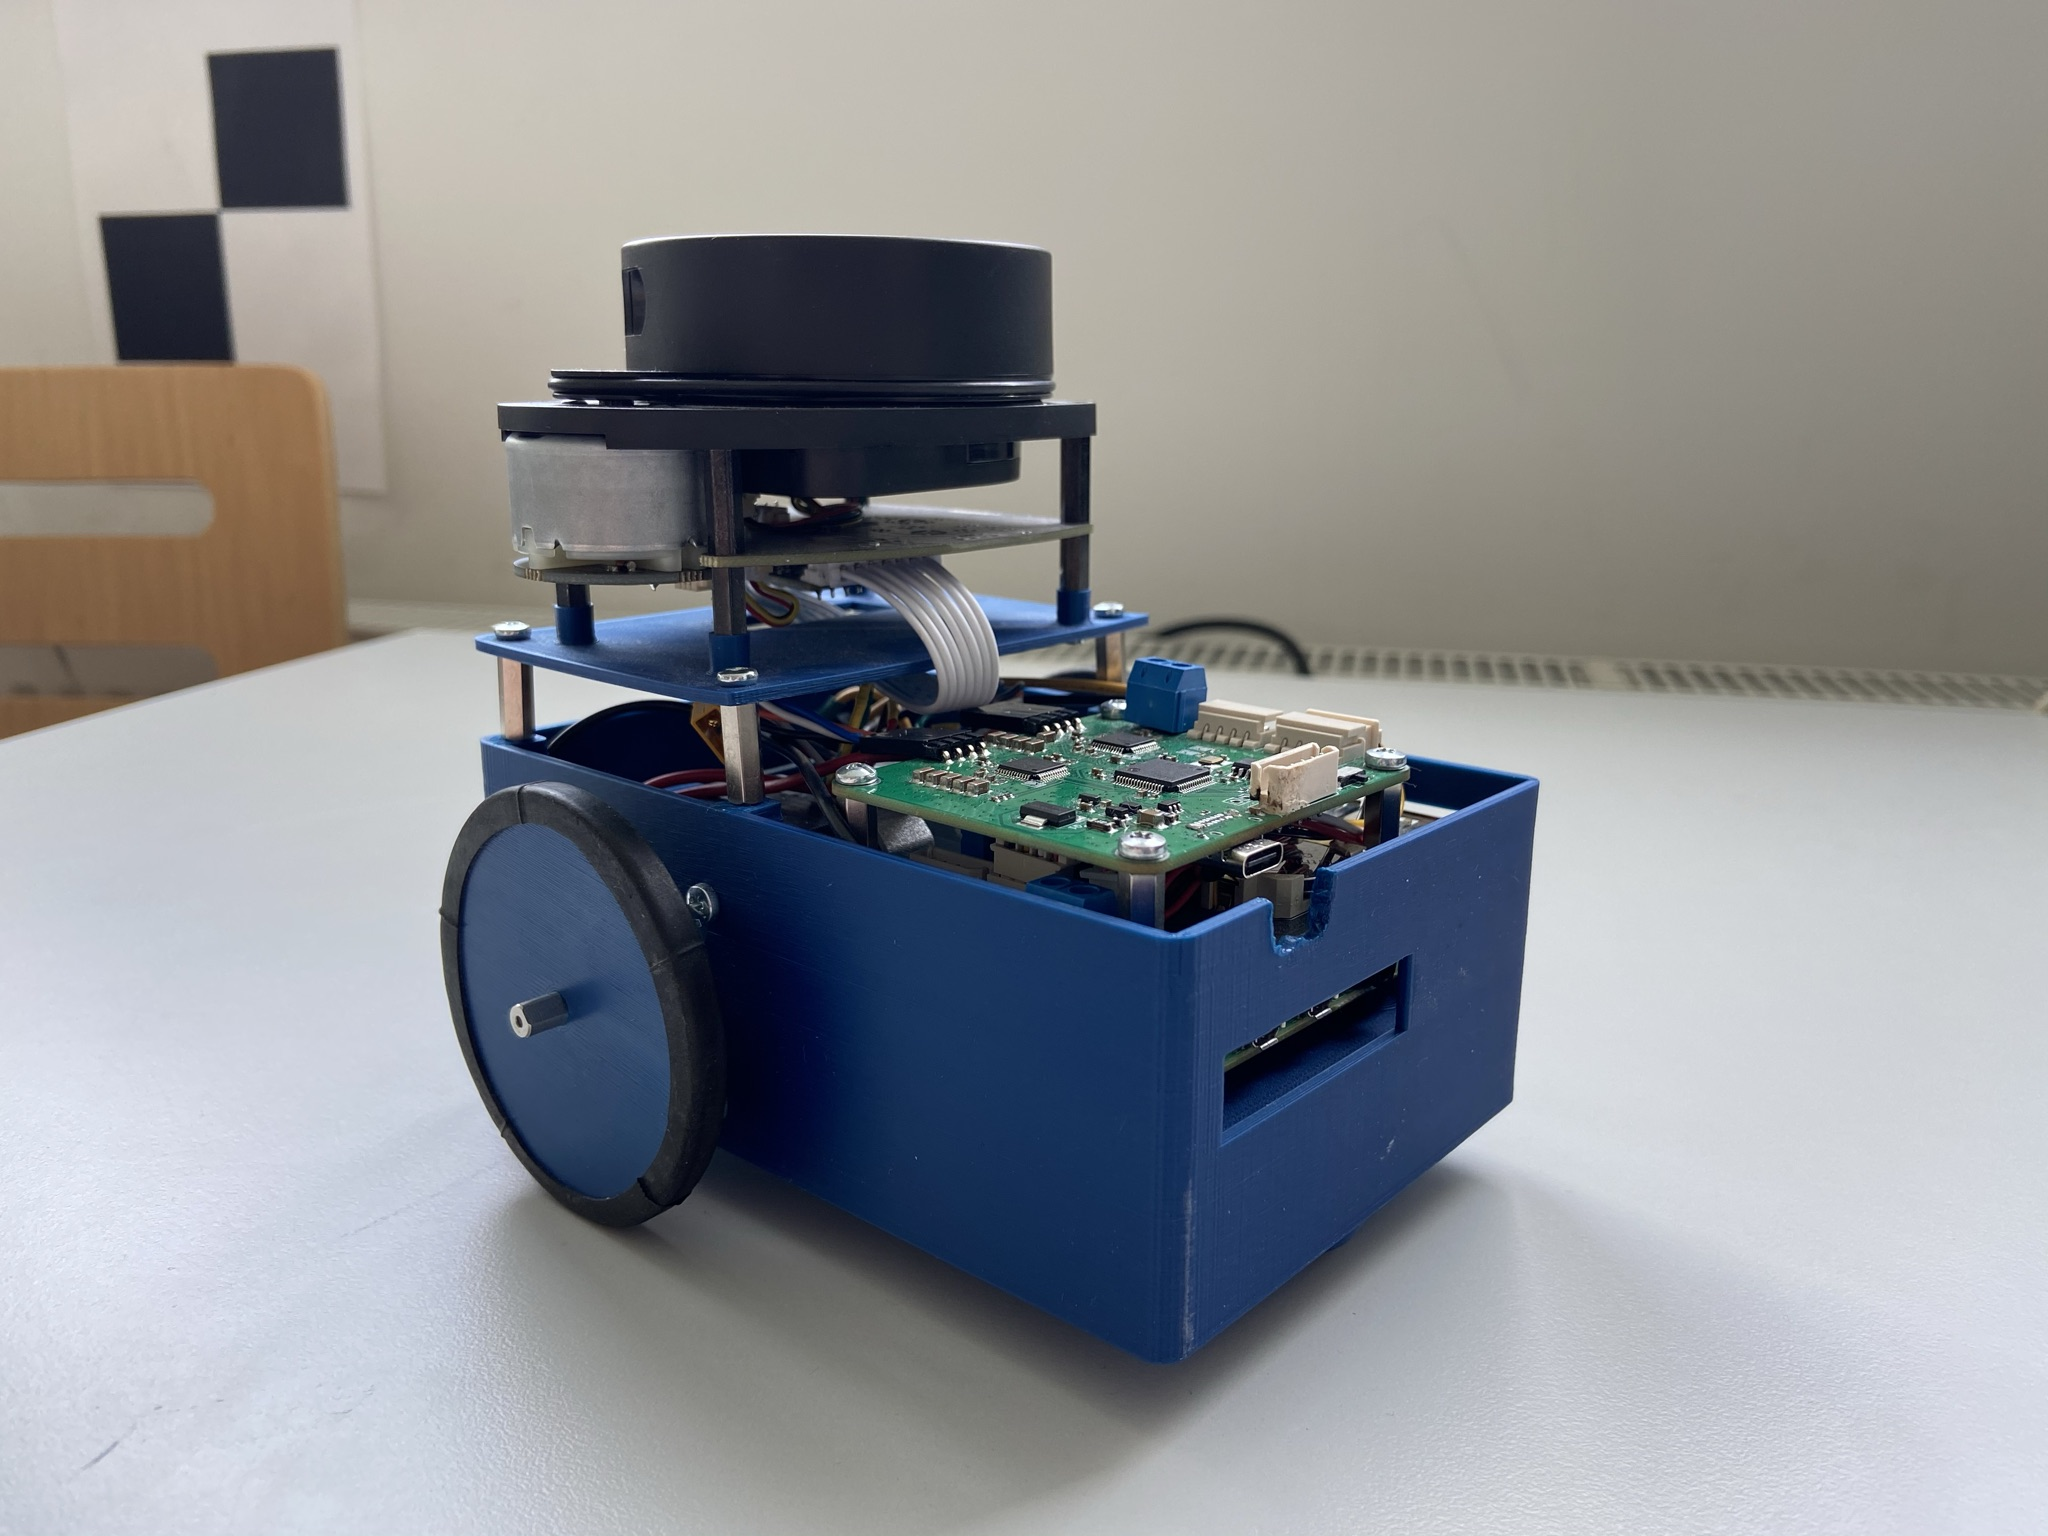
\includegraphics[width=0.7\textwidth]{obrazky/map_bot}
    \caption{The MAP-bot robot - the first demonstration of the SM4 stepper motor controller.}
    \label{fig:map_bot}
\end{figure}

As part of the demonstration, the Raspberry Pi SBC controls the robot to move forward, backward and rotate via CANOpen control of the SM4 stepper motor controller.

\section{Demonstration \#2 - Linear Rail Actuator for Camera Movement}
\label{sec:dem2}
